% -----------------------------------------------------------------------
% NOTE: Blue {\color{blue}[...]} comments and \st{} strikethroughs are
% co-author revision notes to be addressed before submission.
% See quality_reports/plans/2026-05-17_financial-cycle-project-setup.md
% for the full list of open issues.
% -----------------------------------------------------------------------

\subsection{Estimation results}

The financial cycle indicator is derived from a dynamic factor model estimated separately for each country, yielding country-specific measures of the financial cycle. In all countries, standard information criteria select a single common factor ($r = 1$), consistent with the objective of capturing the dominant co-movement among the variables. In practice, the estimated factor is closely related to the first principal component of the data, which explains the largest share of their joint variation. To determine the lag order of the factor dynamics, we fit a VAR model to the PCA-estimated factors and select the number of lags based on standard information criteria, which point to $p = 4$ across all countries. We adopt this lag length uniformly across all three estimators (PCA, QML, and the two-step procedure) to ensure comparability of results.

\paragraph{Goodness of fit.}

Figure~\ref{fig:var_exp} reports the proportion of total variance explained by the first factor for each country. The dashed horizontal line represents the cross-country average, showing that the first factor accounts for approximately 44\% of the total variance on average. In some countries, this share exceeds 50\%, indicating that a single-factor representation provides a reasonably good summary of the common dynamics in the data.

\begin{figure}[htbp]
    \centering
    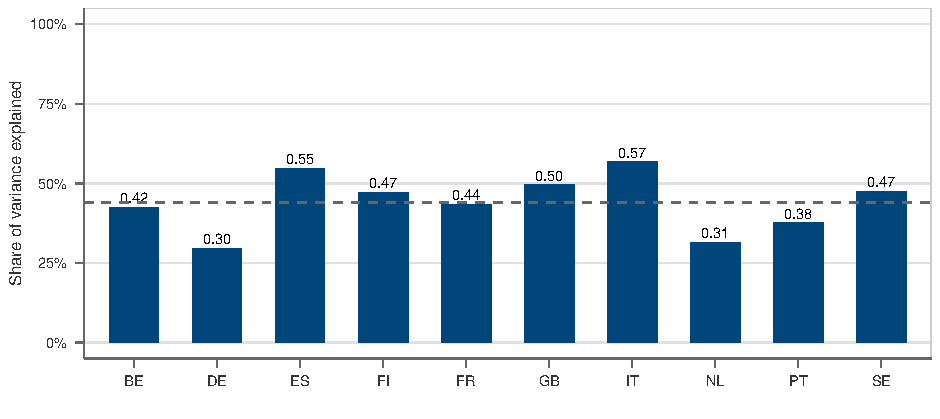
\includegraphics[width=1\linewidth]{../Figures/var_exp.pdf}
    \caption{Share of total variance explained by the first factor}
    \caption*{\footnotesize \textbf{Notes:} The figure reports the share of total variance explained by the estimated factor of the dynamic factor model estimated separately for each country. The dashed horizontal line indicates the cross-country average. All variables are expressed in 2-year growth rates (2-year differences for bond spreads), filtered to remove low-frequency components, and standardised prior to estimation.}
    \label{fig:var_exp}
\end{figure}

Table~\ref{tab:r2} reports the $R^2$ values obtained by regressing each variable on the estimated common component, for all countries in the sample. These values provide a simple measure of how closely each variable co-moves with the financial cycle indicator. The results show that the estimated factor explains a large share of the variation in credit to non-financial corporations, the debt service ratio, and the credit-to-GDP ratio. This finding suggests that the common factor is primarily driven by variables related to credit and indebtedness, which are central to the build-up of cyclical systemic risk.

By contrast, the explanatory power of the factor is generally lower for share prices and sovereign bond spreads, indicating that these variables co-move less systematically with the rest of the dataset. One interpretation is that these series are more strongly influenced by country-specific shocks, global factors, or abrupt changes in market sentiment, which are not fully captured by a single common factor. This pattern is broadly consistent with \citet{drehmann2012characterising}, who emphasise the central role of credit variables in characterising the financial cycle. At the same time, our results suggest that house prices play a more heterogeneous role across countries and, on average, contribute less to the common factor than credit-based indicators.

Some very low $R^2$ values also stand out in Table~\ref{tab:r2}, particularly for share prices in Spain, Germany, and the Netherlands, and for house prices in Portugal, Germany, and the Netherlands. These cases likely reflect the fact that, after the transformations and filtering applied to the data, the corresponding series display relatively weak co-movement with the other variables entering the model. In such cases, a single common factor naturally attributes little explanatory power to those series. This does not imply that these variables are unimportant for financial stability in those countries; rather, it indicates that their cyclical dynamics are less aligned with the dominant common component identified by the model.

\begin{table}[htbp]
  \centering
  \caption{$R^2$ of the first factor across variables}
  \label{tab:r2}
  \small
  \setlength{\tabcolsep}{5pt}
  \begin{tabular}{l *{7}{S[table-format=1.2]}}
  \toprule
  \textbf{Country}
    & \multicolumn{1}{c}{\textbf{\shortstack[c]{Credit\\NFC}}}
    & \multicolumn{1}{c}{\textbf{\shortstack[c]{Credit\\HH}}}
    & \multicolumn{1}{c}{\textbf{\shortstack[c]{House\\prices}}}
    & \multicolumn{1}{c}{\textbf{\shortstack[c]{Share\\prices}}}
    & \multicolumn{1}{c}{\textbf{DSR}}
    & \multicolumn{1}{c}{\textbf{\shortstack[c]{Credit-\\to-GDP}}}
    & \multicolumn{1}{c}{\textbf{\shortstack[c]{Bond\\spread}}} \\
  \midrule
  BE & 0.85 & 0.15 & 0.10 & 0.12 & 0.84 & 0.84 & 0.07 \\
  DE & 0.66 & 0.08 & 0.02 & 0.00 & 0.60 & 0.66 & 0.06 \\
  ES & 0.88 & 0.90 & 0.48 & 0.00 & 0.82 & 0.75 & 0.01 \\
  FI & 0.83 & 0.31 & 0.06 & 0.21 & 0.89 & 0.71 & 0.29 \\
  FR & 0.83 & 0.43 & 0.27 & 0.01 & 0.75 & 0.70 & 0.05 \\
  GB & 0.76 & 0.72 & 0.39 & 0.02 & 0.81 & 0.76 & 0.01 \\
  IT & 0.88 & 0.80 & 0.68 & 0.06 & 0.70 & 0.70 & 0.16 \\
  NL & 0.62 & 0.02 & 0.04 & 0.00 & 0.76 & 0.70 & 0.05 \\
  PT & 0.87 & 0.33 & 0.00 & 0.02 & 0.58 & 0.72 & 0.12 \\
  SE & 0.81 & 0.66 & 0.27 & 0.04 & 0.75 & 0.78 & 0.01 \\
  \midrule
  \textbf{Average}
    & {\textbf{0.80}} & {\textbf{0.44}} & {\textbf{0.23}} & {\textbf{0.05}}
    & {\textbf{0.75}} & {\textbf{0.73}} & {\textbf{0.08}} \\
  \bottomrule
  \end{tabular}
  \smallskip
  \begin{minipage}{\linewidth}
    \footnotesize\textit{Notes:} The table reports the $R^2$ from regressing each variable on the estimated common factor of the dynamic factor model, computed separately for each country. All variables are expressed in 2-year growth rates (2-year differences for bond spreads), filtered to remove low-frequency components, and standardised prior to estimation. Higher values indicate stronger co-movement with the common factor. HH denotes households.
  \end{minipage}
\end{table}

\paragraph{Evolution of the financial cycle across countries.}

Figure~\ref{fig:factor_median} reports the median financial cycle indicator across the countries in the sample (results for individual countries are provided in Appendix~\ref{AppendixA}). Estimates are obtained using three alternative methods: principal components (PCA), quasi-maximum likelihood (QML), and the two-step estimator (TSTEP). The figure also displays the interquartile range (25th--75th percentiles), capturing the cross-country dispersion of the financial cycle across estimators. The similarity of the estimated cycles across methods indicates that the main features of the financial cycle are robust to the choice of estimator.

\begin{figure}[htbp]
    \centering
    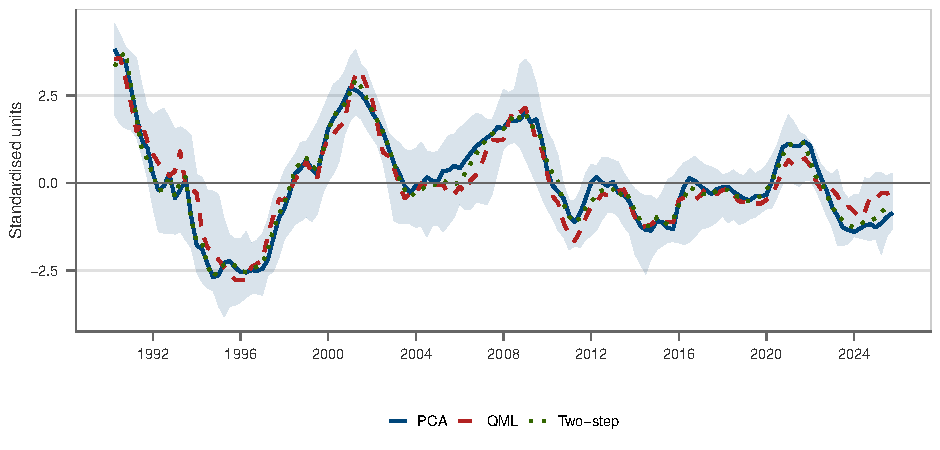
\includegraphics[width=1\linewidth]{../Figures/factor_medians.pdf}
    \caption{Median financial cycle indicator across countries}
    \caption*{\footnotesize \textbf{Notes:} The figure shows the median financial cycle indicator across countries, together with the interquartile range (25th--75th percentiles). Results are reported for three estimation methods: principal components (PCA), quasi-maximum likelihood (QML), and two-step estimator (TSTEP). The shaded area represents cross-country dispersion across all estimators.}
    \label{fig:factor_median}
\end{figure}

The results show that the financial cycle is characterised by medium-term fluctuations \citep{borio2014financial, drehmann2012characterising}, with phases lasting on the order of 8 to 12 years. This distinguishes the financial cycle from the business cycle, which typically operates at higher frequencies \citep{claessens2012business}. Over the sample period, the financial cycle exhibits three prominent peaks: in the early 2000s, in the run-up to the GFC in 2007--2008, and following the COVID-19 shock. These episodes coincide with periods of strong credit expansion, rising leverage, and increasing systemic risk.

Following the GFC, the financial cycle enters a prolonged subdued phase, characterised by lower amplitude and reduced variability. This pattern is consistent with the post-crisis regulatory environment, which includes tighter capital requirements, constraints on leverage, and the broader use of macroprudential policy tools aimed at containing the build-up of systemic risk.

The post-COVID period is marked by a sharp but short-lived expansion of the financial cycle, reflecting the unprecedented scale of fiscal and monetary support measures. This phase is associated with rapid credit growth, abundant liquidity, and rising asset prices. However, from 2022 onwards, the financial cycle contracts as inflationary pressures intensify and monetary policy tightens globally. The resulting increase in interest rates leads to a deterioration in financing conditions and a slowdown in credit dynamics.

Overall, these results highlight the close interaction between macroeconomic conditions, policy interventions, and the financial cycle. In particular, they illustrate how expansionary policies can amplify financial dynamics, while monetary tightening and regulatory constraints can contribute to their reversal.

\subsection{Decomposition}

\paragraph{Approach.}

The factor estimates can be further decomposed into contributions from the underlying variables, providing a clearer understanding of the main drivers of the financial cycle. The decomposition is performed in-sample as follows. We regress the estimated factor (obtained using the PCA estimator) on the standardised variables without a constant term. Each variable's contribution is then computed as the product of its normalised weight, defined as the absolute value of the corresponding regression coefficient divided by the sum of all absolute coefficients, and its observed value. An exception is made for sovereign bond spreads, whose weight retains the sign of the regression coefficient: because spread compression (declining spreads) signals financial cycle expansion, a negative coefficient on spreads correctly captures the inverse relationship between spread levels and the financial cycle, ensuring that this variable's contribution is correctly attributed. 
\paragraph{Empirical evidence.}

Figure~\ref{fig:dec_graph} illustrates the decomposition of the median of the financial cycle indicator across the set of countries in the sample (results for individual countries are available in Appendix~\ref{AppendixB}). The financial cycle shows a pronounced build-up in the early 2000s, primarily driven by strong growth in household credit and non-financial corporations credit, alongside rising DSR and credit-to-GDP ratios. This expansion is followed by a sharp contraction during the mid-2000s, as credit growth decelerates and the financial cycle indicator approaches its long-term average.

A significant increase occurs leading up to the 2007--2008 GFC, largely due to an increase in the growth of credit to households and increasing house prices. The onset of the GFC triggers a sharp and prolonged downturn in the financial cycle, a decline further exacerbated by the European sovereign debt crisis in 2010. During this period, the contribution of most variables, including credit indicators and house prices, turns negative, reflecting widespread deleveraging and financial distress across European economies.

In the second half of the 2010s, the financial cycle stabilises at relatively subdued levels, as credit growth remains weak despite gradual improvements. Notably, house prices emerge as a more significant driver of the financial cycle during this phase, reflecting growing overvaluation concerns in certain European housing markets. A renewed recovery is observed following the COVID-19 shock, driven by credit expansion and increased liquidity from unprecedented fiscal and monetary support.

Around 2022, the financial cycle enters a renewed downturn as global inflation accelerates and central banks implement rapid monetary tightening. The decline in the credit-to-GDP ratio and house prices weighs significantly on the financial cycle.

Overall, the decomposition underscores that while credit growth and leverage measures remain the primary drivers of financial cycle fluctuations, asset prices and interest rate spreads have played a significant role during specific periods. These insights can enhance the monitoring of financial cycles, help identify emerging trends and risks, and ultimately inform macroprudential policy.

\begin{figure}[htbp]
    \centering
    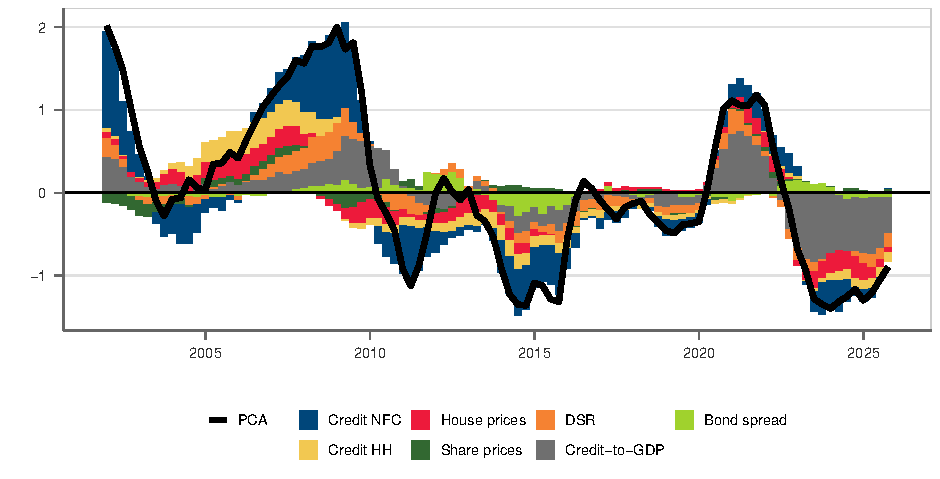
\includegraphics[width=1\linewidth]{../Figures/dec_graph.pdf}
    \caption{Decomposition of the median financial cycle indicator across countries}
    \caption*{\footnotesize \textbf{Notes:} The figure shows the in-sample decomposition of the median financial cycle indicator across countries. Each variable's contribution is the product of its observed (standardised) value and a normalised weight derived from a zero-intercept regression of the estimated factor on all variables. Weights are proportional to the absolute regression coefficients, except for sovereign bond spreads, which retain the sign of the coefficient to correctly reflect that spread compression signals financial cycle expansion. Contributions are scaled to sum to the estimated factor.}
    \label{fig:dec_graph}
\end{figure}

\subsection{Identification of a neutral risk environment}

\paragraph{Approach.}

A neutral risk environment corresponds to a state in which cyclical systemic risk is neither elevated nor subdued. It is typically associated with moderate credit growth, stable asset price dynamics, and financial conditions that do not signal the build-up or materialisation of imbalances. In such periods, vulnerabilities evolve in line with underlying economic fundamentals, without clear signs of overheating or stress.

To operationalise this concept, we adopt a quantitative approach based on the financial cycle indicator. Specifically, we define a neutral regime as periods in which the indicator remains close to its long-term average. Drawing on the asymptotic distribution theory of the principal components estimator for the common factor, we construct confidence bands around the estimated financial cycle. These bands provide a statistical benchmark to identify significant deviations from typical conditions. Periods in which the indicator lies within the confidence bands are classified as neutral, while deviations outside these bands signal either elevated or subdued cyclical systemic risk.

\paragraph{Empirical evidence.}

Figure~\ref{fig:ci_medians} illustrates this approach using the median financial cycle indicator across countries (country-specific results are reported in Appendix~\ref{AppendixC}). The shaded area represents the 95\% confidence bands, while the dashed lines denote the time-averaged upper and lower confidence bounds, which serve as constant thresholds for regime classification. This framework allows for a clear classification of financial cycle phases. Elevated regimes correspond to periods in which the indicator exceeds the upper bound, signalling heightened systemic risk. Subdued regimes are identified when the indicator falls below the lower bound, typically reflecting the materialisation of risk and subsequent deleveraging. Neutral regimes correspond to periods in which the indicator remains within the confidence bands.

For the median across countries, the results identify elevated financial cycle phases in the early 2000s and in the run-up to the GFC, coinciding with strong credit expansion and rising asset prices. In contrast, the period following the European sovereign debt crisis is characterised by a subdued regime, reflecting weak credit growth and subdued financial activity. From around 2016 onwards, the financial cycle gradually converges towards a neutral regime. As of 2025~Q3, the most recent observations suggest that the financial cycle has moved back into a subdued phase.

\begin{figure}[htbp]
    \centering
    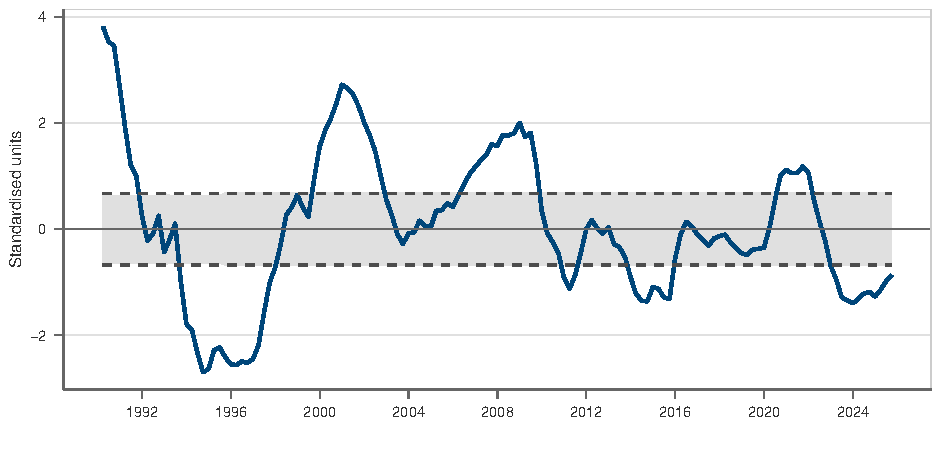
\includegraphics[width=1\linewidth]{../Figures/ci_medians.pdf}
    \caption{Financial cycle indicator and 95\% confidence intervals}
    \caption*{\footnotesize \textbf{Notes:} The figure displays the median financial cycle indicator across countries together with 95\% confidence bands based on the asymptotic distribution of the estimated factor. The shaded area represents the time-varying confidence bands, while the dashed lines denote the time-averaged upper and lower bounds used as constant thresholds for regime classification. Values above (below) the upper (lower) dashed line indicate statistically significant deviations associated with elevated (subdued) cyclical systemic risk.}
    \label{fig:ci_medians}
\end{figure}

\paragraph{Cross-country analysis of financial cycle regimes.}

Extending this framework across countries, Figure~\ref{fig:regimes_graph} classifies financial cycle conditions into subdued, neutral, and elevated regimes over time. Subdued regimes are prevalent in the mid-to-late 1990s and during the post-GFC period, reflecting deleveraging and weak credit dynamics. Elevated regimes are concentrated in the early 2000s and in the run-up to the GFC, consistent with the build-up of systemic risk. Following the COVID-19 shock, many countries temporarily transition towards neutral conditions, supported by expansionary fiscal and monetary policies. Since 2022, however, several countries have returned to subdued regimes as tighter monetary policy and higher interest rates weigh on credit growth and financial activity.

\begin{figure}[htbp]
    \centering
    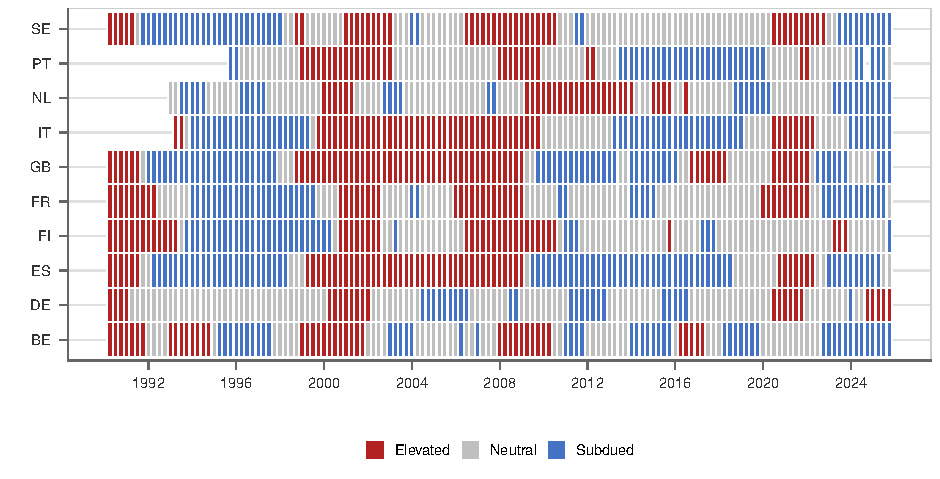
\includegraphics[width=1\linewidth]{../Figures/regimes_graph.pdf}
    \caption{Financial cycle regimes across countries}
    \caption*{\footnotesize \textbf{Notes:} The figure classifies financial cycle conditions across countries into subdued, neutral, and elevated regimes based on the position of the financial cycle indicator relative to its estimated confidence bands. Each bar represents the share of countries in each regime at a given point in time.}
    \label{fig:regimes_graph}
\end{figure}

\paragraph{Policy implications.}

The calibration of the countercyclical capital buffer (CCyB) is subject to considerable uncertainty, as the build-up of cyclical systemic risk is difficult to measure in real time. In practice, this raises the risk of delayed or insufficient policy action, as well as the possibility of underestimating vulnerabilities during periods of apparent stability.

In response to these challenges, the concept of a positive neutral CCyB has gained prominence. As of November 2025, 17 macroprudential authorities in the European Economic Area (EEA) have implemented a positive neutral CCyB framework. A positive neutral CCyB refers to a capital buffer maintained when risks are assessed as neither elevated nor subdued, ensuring that banks hold releasable capital in normal times. Evidence from the COVID-19 episode shows that the release of such buffers supports lending and mitigates procyclical deleveraging, alleviating concerns about banks' reluctance to use capital buffers \citep{avezum2024assessment, berrospide2021used, ecbesrb2026usability}.

Our approach enables the identification of periods in which cyclical systemic risks are neither building up nor materialising. By assessing deviations in the financial cycle, constructed as deviations of underlying indicators from their long-term averages, it provides a benchmark for evaluating when risks lie within a neutral range. In this context, the framework offers a transparent and operational tool to inform the calibration of the neutral level of the CCyB.

\subsection{Identification of financial crises}

As documented by \citet{borio2014financial}, one defining feature of financial cycles is that they tend to be closely associated with systemic banking crises. This link suggests that a good measure of the financial cycle can be used as a leading indicator to signal the build-up of risk that may culminate in a financial crisis. In this section, we investigate the early-warning properties of our proposed measure of the financial cycle.

Our analysis is conducted using the systemic banking crisis dataset constructed by \citet{lo2017new} for European countries. A crisis, as defined by this dataset, refers to a period during which the financial system served as a source or amplifier of economic shocks, financial intermediaries faced significant distress or collapse, and substantial crisis management policies were implemented.

\paragraph{Set-up of the early-warning analysis.}
We estimate country-specific logit regressions to assess the build-up of systemic risk ahead of banking crises. The dependent variable is a binary vulnerability indicator that takes the value one during the five to twelve quarters preceding a systemic banking crisis and zero otherwise. This definition emphasises the objective of detecting early signs of financial imbalances, rather than predicting the exact timing of a crisis. This distinction is important, as macroprudential policy must be preemptive to be effective. Moreover, there are implementation lags that constrain policy responsiveness. For example, the CCyB includes a one-year phase-in period, allowing banks time to adjust to new capital requirements. As a result, signals issued less than a year before a crisis are likely too late for an effective policy response. The focus is therefore on identifying vulnerabilities early enough to enable timely intervention.

As independent variable, we consider the financial cycle measure obtained in the context of a dynamic factor model estimated with different estimators. Our analysis is purely univariate as we do not consider additional variables or lags of the indicator. To benchmark our results, we use the Basel gap, calculated as the cyclical component of the total credit-to-GDP ratio derived from a recursive HP filter with a smoothing parameter of 400,000. The Basel gap is chosen as the benchmark indicator because it is widely considered as a leading univariate signal of systemic financial crises. It serves as the recommended reference indicator for activating the countercyclical capital buffer under the guidance of the Basel Committee on Banking Supervision.

We use two measures of accuracy in the early-warning exercise: the area under the receiver operating characteristic curve (AUROC); and the usefulness index proposed by \citet{alessi2011quasi}. The AUROC is a global measure of accuracy that relates the false positive rate (noise ratio) to the true positive rate (signal ratio) for every possible threshold value applied to the predicted probabilities from the logit regression. \citet{hanley1982meaning} show that the AUROC can be interpreted as the probability of correctly classifying zeros and ones.

The usefulness index represents a measure of the gain from following the model relative to disregarding it, adjusted for the preferences of policymakers regarding type~I (failing to signal a financial crisis, denoted by $T_1$) and type~II (``false alarms'', denoted by $T_2$) errors. The index is defined as:
\begin{equation}
    U = \frac{\min[\theta;\, 1- \theta] - L(\theta)}{\min[\theta;\, 1- \theta]},
\end{equation}
where $L(\theta)$ denotes the policymaker's loss function:
\begin{equation}
   L(\theta) = \theta T_1 + (1- \theta) T_2.
\end{equation}
The parameter $\theta$ controls policymaker preferences. A value of $\theta$ below 0.5 indicates that the policymaker is less averse to missing a crisis signal than to receiving a false alarm. Because the policymaker can always achieve a loss of $\min[\theta; 1-\theta]$ by disregarding the indicator, the usefulness index compares the loss under the logit model against the loss of ignoring it. We consider two preference specifications: balanced preferences ($\theta = 0.5$), following \citet{lang2019anticipating}, and crisis-averse preferences ($\theta = 0.7$), which assign greater weight to type~I errors (failing to signal a crisis).

Finally, we consider the full sample used in the previous analysis, with two exceptions. First, Finland is excluded from the early-warning exercise, as it did not experience a systemic banking crisis during the sample period (1995~Q3--2025~Q3); its major banking crisis occurred in the early 1990s, prior to the start of the sample. Second, we exclude the crisis periods themselves from the sample used to estimate the logit models. This follows the recommendation of \citet{bussiere2006towards}, who show that early-warning model performance can be distorted by the disorderly and volatile adjustment of explanatory variables following the onset of a crisis. To avoid this so-called post-crisis bias, we focus only on the pre-crisis and tranquil periods in the estimation.

\paragraph{In-sample exercise.}
The results for all countries, presented in Table~\ref{tab:ew_in_sample}, show that the financial cycle indicator constructed using a dynamic factor model has good early-warning properties. On average, the DFM-based indicators outperform the Basel gap in terms of AUROC (0.68 for PCA versus 0.55 for BG), while delivering a comparable usefulness index under both balanced ($\theta=0.5$) and crisis-averse ($\theta=0.7$) preferences. The advantage is particularly marked for Germany, where the Basel gap delivers near-zero usefulness under crisis-averse preferences (0.02), while the PCA-based indicator remains informative (0.13). Among estimators, PCA and the two-step estimator perform similarly, while QML exhibits more variation across countries.

\begin{table}[htbp]
  \centering
  \caption{In-sample early-warning exercise}
  \label{tab:ew_in_sample}
  \footnotesize
  \setlength{\tabcolsep}{2pt}
  \begin{tabular}{l @{\hspace{1em}}
                  S[table-format=1.2] S[table-format=1.2] S[table-format=1.2] S[table-format=1.2]
                  @{\hspace{1em}}
                  S[table-format=1.2] S[table-format=1.2] S[table-format=1.2] S[table-format=1.2]
                  @{\hspace{1em}}
                  S[table-format=1.2] S[table-format=1.2] S[table-format=1.2] S[table-format=1.2]}
  \toprule
        & \multicolumn{4}{c}{\textbf{AUROC}}
        & \multicolumn{4}{c}{\textbf{Usefulness ($\theta = 0.5$)}}
        & \multicolumn{4}{c}{\textbf{Usefulness ($\theta = 0.7$)}} \\
  \cmidrule(lr){2-5}\cmidrule(lr){6-9}\cmidrule(lr){10-13}
  \textbf{Country}
        & {\textbf{PCA}} & {\textbf{QML}} & {\textbf{TSTEP}} & {\textbf{BG}}
        & {\textbf{PCA}} & {\textbf{QML}} & {\textbf{TSTEP}} & {\textbf{BG}}
        & {\textbf{PCA}} & {\textbf{QML}} & {\textbf{TSTEP}} & {\textbf{BG}} \\
  \midrule
  BE & 0.51 & 0.65 & 0.57 & 0.51 & 0.20 & 0.20 & 0.21 & 0.26 & 0.12 & 0.12 & 0.13 & 0.15 \\
  DE & 0.76 & 0.85 & 0.73 & 0.36 & 0.25 & 0.26 & 0.25 & 0.08 & 0.13 & 0.13 & 0.11 & 0.02 \\
  ES & 1.00 & 0.93 & 0.99 & 0.60 & 0.49 & 0.46 & 0.48 & 0.28 & 0.29 & 0.27 & 0.29 & 0.17 \\
  FR & 0.78 & 0.48 & 0.64 & 0.61 & 0.30 & 0.16 & 0.22 & 0.30 & 0.17 & 0.09 & 0.13 & 0.18 \\
  GB & 0.72 & 0.77 & 0.77 & 0.63 & 0.29 & 0.29 & 0.30 & 0.27 & 0.18 & 0.18 & 0.18 & 0.16 \\
  IT & 0.67 & 0.75 & 0.68 & 0.55 & 0.18 & 0.27 & 0.21 & 0.27 & 0.11 & 0.06 & 0.13 & 0.16 \\
  NL & 0.42 & 0.62 & 0.45 & 0.53 & 0.07 & 0.19 & 0.10 & 0.27 & 0.04 & 0.11 & 0.06 & 0.16 \\
  PT & 0.54 & 0.66 & 0.53 & 0.53 & 0.24 & 0.24 & 0.20 & 0.25 & 0.15 & 0.14 & 0.12 & 0.15 \\
  SE & 0.73 & 0.57 & 0.67 & 0.64 & 0.26 & 0.10 & 0.18 & 0.32 & 0.14 & 0.06 & 0.11 & 0.19 \\
  \midrule
  \textbf{Avg}
       & {\textbf{0.68}} & {\textbf{0.70}} & {\textbf{0.67}} & {\textbf{0.55}}
       & {\textbf{0.25}} & {\textbf{0.24}} & {\textbf{0.24}} & {\textbf{0.26}}
       & {\textbf{0.15}} & {\textbf{0.13}} & {\textbf{0.14}} & {\textbf{0.15}} \\
  \bottomrule
  \end{tabular}
  \smallskip
  \begin{minipage}{\linewidth}
    \footnotesize\textit{Notes:} PCA, QML, and TSTEP refer to estimates of the financial cycle indicator obtained using the principal components, quasi-maximum likelihood, and two-step estimators, respectively. BG denotes the credit-to-GDP gap (Basel gap). AUROC is the area under the receiver operating characteristic curve. The usefulness index is computed following \citet{alessi2011quasi}; $\theta$ weights type~I errors (failing to signal a crisis) against type~II errors (false alarms). A value of $\theta = 0.5$ implies balanced preferences; $\theta = 0.7$ implies crisis-averse preferences (70\% weight on missed crises). The maximum attainable usefulness is $\min(\theta,1{-}\theta)$, equal to 0.50 for $\theta=0.5$ and 0.30 for $\theta=0.7$. Finland is excluded as it did not experience a systemic banking crisis during the sample period (1995~Q3--2025~Q3); its major banking crisis occurred in the early 1990s, prior to the start of the sample.
  \end{minipage}
\end{table}

\paragraph{Simulated out-of-sample exercise.}
We also conduct an out-of-sample exercise focusing on the GFC to assess the early-warning properties of the financial cycle indicator. Evaluating such properties for this period is particularly challenging due to the very low frequency of systemic banking crises. Despite this constraint, the credibility of an early-warning model depends on its ability to detect, in real time, the build-up of financial imbalances preceding a crisis.

To address this issue, we follow an approach similar to \citet{alessi2018identifying} and examine the model's predictions as of mid-2006, using only data available up to the second quarter of that year. Crucially, this exercise excludes any knowledge of the subsequent GFC, ensuring a realistic assessment of the model's practical utility. To broaden the set of countries for which out-of-sample predictions can be generated, we also include ``residual events'' as defined by \citet{detken2014operationalising}. Residual events are episodes in which domestic financial imbalances reached levels consistent with systemic stress, but an outright crisis was averted, typically because policy interventions or favourable external conditions dampened the credit cycle at a critical juncture. Treating these near-miss episodes as crisis signals allows us to draw on a richer set of early-warning observations.

The exercise is conducted in pseudo-real time, meaning that all transformations are based solely on information available up to each point in time. However, we acknowledge two simplifying assumptions: first, we rely on final revised data rather than vintages, and second, we assume no publication lag, meaning observations for a given period are assumed to be available immediately. The procedure involves estimating the dynamic factor model using data up to 2006~Q1. We then perform a logit regression of the vulnerability indicator on the financial cycle indicator and use the resulting model to predict the probability of a financial crisis occurring within one year. This process is repeated for each quarter through 2009~Q1.

\begin{figure}[htbp]
    \centering
    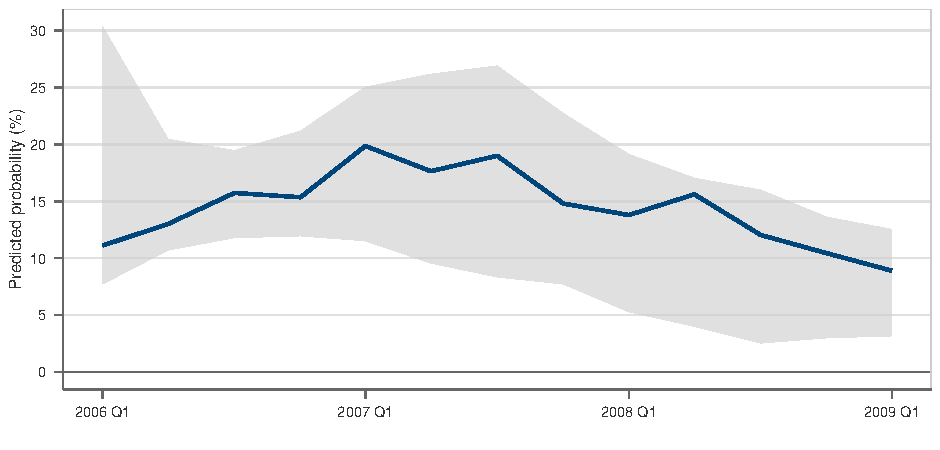
\includegraphics[width=1\linewidth]{../Figures/oos_graph.pdf}
    \caption{Simulated out-of-sample predicted probability of a financial crisis within one year}
    \label{fig:oos_graph}
    \caption*{\footnotesize \textbf{Notes:} The figure reports the median predicted probability of a systemic banking crisis within one year across countries, together with the interquartile range. Predictions are obtained from country-specific logit models estimated in pseudo-real time using only information available up to each point in time. The left dashed vertical line marks the onset of the Euro area recession (2008 Q2); the right dashed vertical line marks the collapse of Lehman Brothers (15 September 2008).}
\end{figure}

Figure~\ref{fig:oos_graph} illustrates the cross-country median of the predicted crisis probabilities alongside the 25th--75th interquartile range. The key finding is the trajectory of the indicator: the estimated median probability of a systemic banking crisis within one year approximately doubles between early 2006 and 2007, rising from approximately 10\% to around 20\%. This sharp increase, generated entirely from information available in real time and without any knowledge of the forthcoming GFC, constitutes a clear and economically meaningful early-warning signal. That the absolute probability level does not exceed 20\% is unsurprising: the logit models are estimated on a sample that had not yet witnessed a crisis of the GFC's magnitude, so the predicted probabilities are naturally anchored to the historical base rate of crisis occurrence. What matters for policy purposes is the signal embedded in the trend. An approximate doubling of the estimated crisis probability in the two years preceding the crisis represents a meaningful early-warning signal for macroprudential policy. These results suggest that even a simple univariate model based on the financial cycle indicator can provide valuable and actionable early-warning signals.
